\subsection{Glyph: \glyph{Nucleic acid feature}}
\label{sec:genetic}

The \emph{nucleic acid feature} represents a fragment of a macromolecule carrying genetic information.
A common use for this construct is to represent a gene or transcript.
The label of this EPN and its \emph{units of information} are often crucial for making the purpose clear to the reader of a map.

\begin{glyphDescription}

\glyphSboTerm
SBO:0000354 ! informational molecule segment

\glyphIncoming
Zero or more \glyph{production} arcs (\sect{production}).

\glyphOutgoing
Zero or more \glyph{consumption} arcs (\sect{consumption}), \glyph{modulation arcs} (\sect{modulations}), \glyph{logic arcs} (\sect{logicArc}), or \glyph{equivalence arcs} (\sect{equivalenceArc}).

\glyphContainer
A \glyph{nucleic acid feature} is represented by a rectangular shape whose bottom half has rounded corners.
This design reminds us that we are fundamentally dealing with a unit of information carried by a macromolecule.

\glyphLabel
A \glyph{nucleic acid feature} is identified by a label that is  a string of characters that may be distributed on several lines to improve readability.
The centre of the label must be placed on the centre of the container.
The label may extend outside of the container.

\glyphAux
A \glyph{nucleic acid feature} can carry one or more \glyph{state variables} that add information about its state (\sect{stateVariable}).
The state of a \glyph{nucleic acid feature} is defined as the list of all its \glyph{state variables}.

A \glyph{nucleic acid feature} can also carry one or more \glyph{units of information} (\sect{unitInfo}).
These can characterise a domain, such as a binding site.
Particular \glyph{units of information} are available for describing the material type (\sect{material-types-cv}) and the conceptual type (\sect{conceptual-types-cv}) of a \glyph{nucleic acid feature}.

Finally, a \glyph{nucleic acid feature} can also carry a \glyph{labelled clone marker} (see \sect{cloneMarker}).

\end{glyphDescription}

\begin{figure}[H]
  \centering
  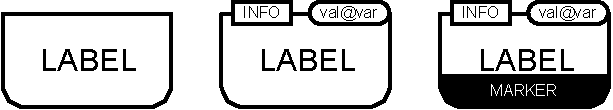
\includegraphics{images/build/genetic_combined}
  \caption{The \PD glyph for \glyph{nucleic acid feature}, shown plain and unadorned on the left, with an additional \glyph{state variable} and a \glyph{unit of information} in the middle, and with a \glyph{labelled clone marker} on the right.}
  \label{fig:genetic}
\end{figure}
